\label{ArchitekturundVerhalten}

%\begin{figure}[!hbt]
%	\centering
%	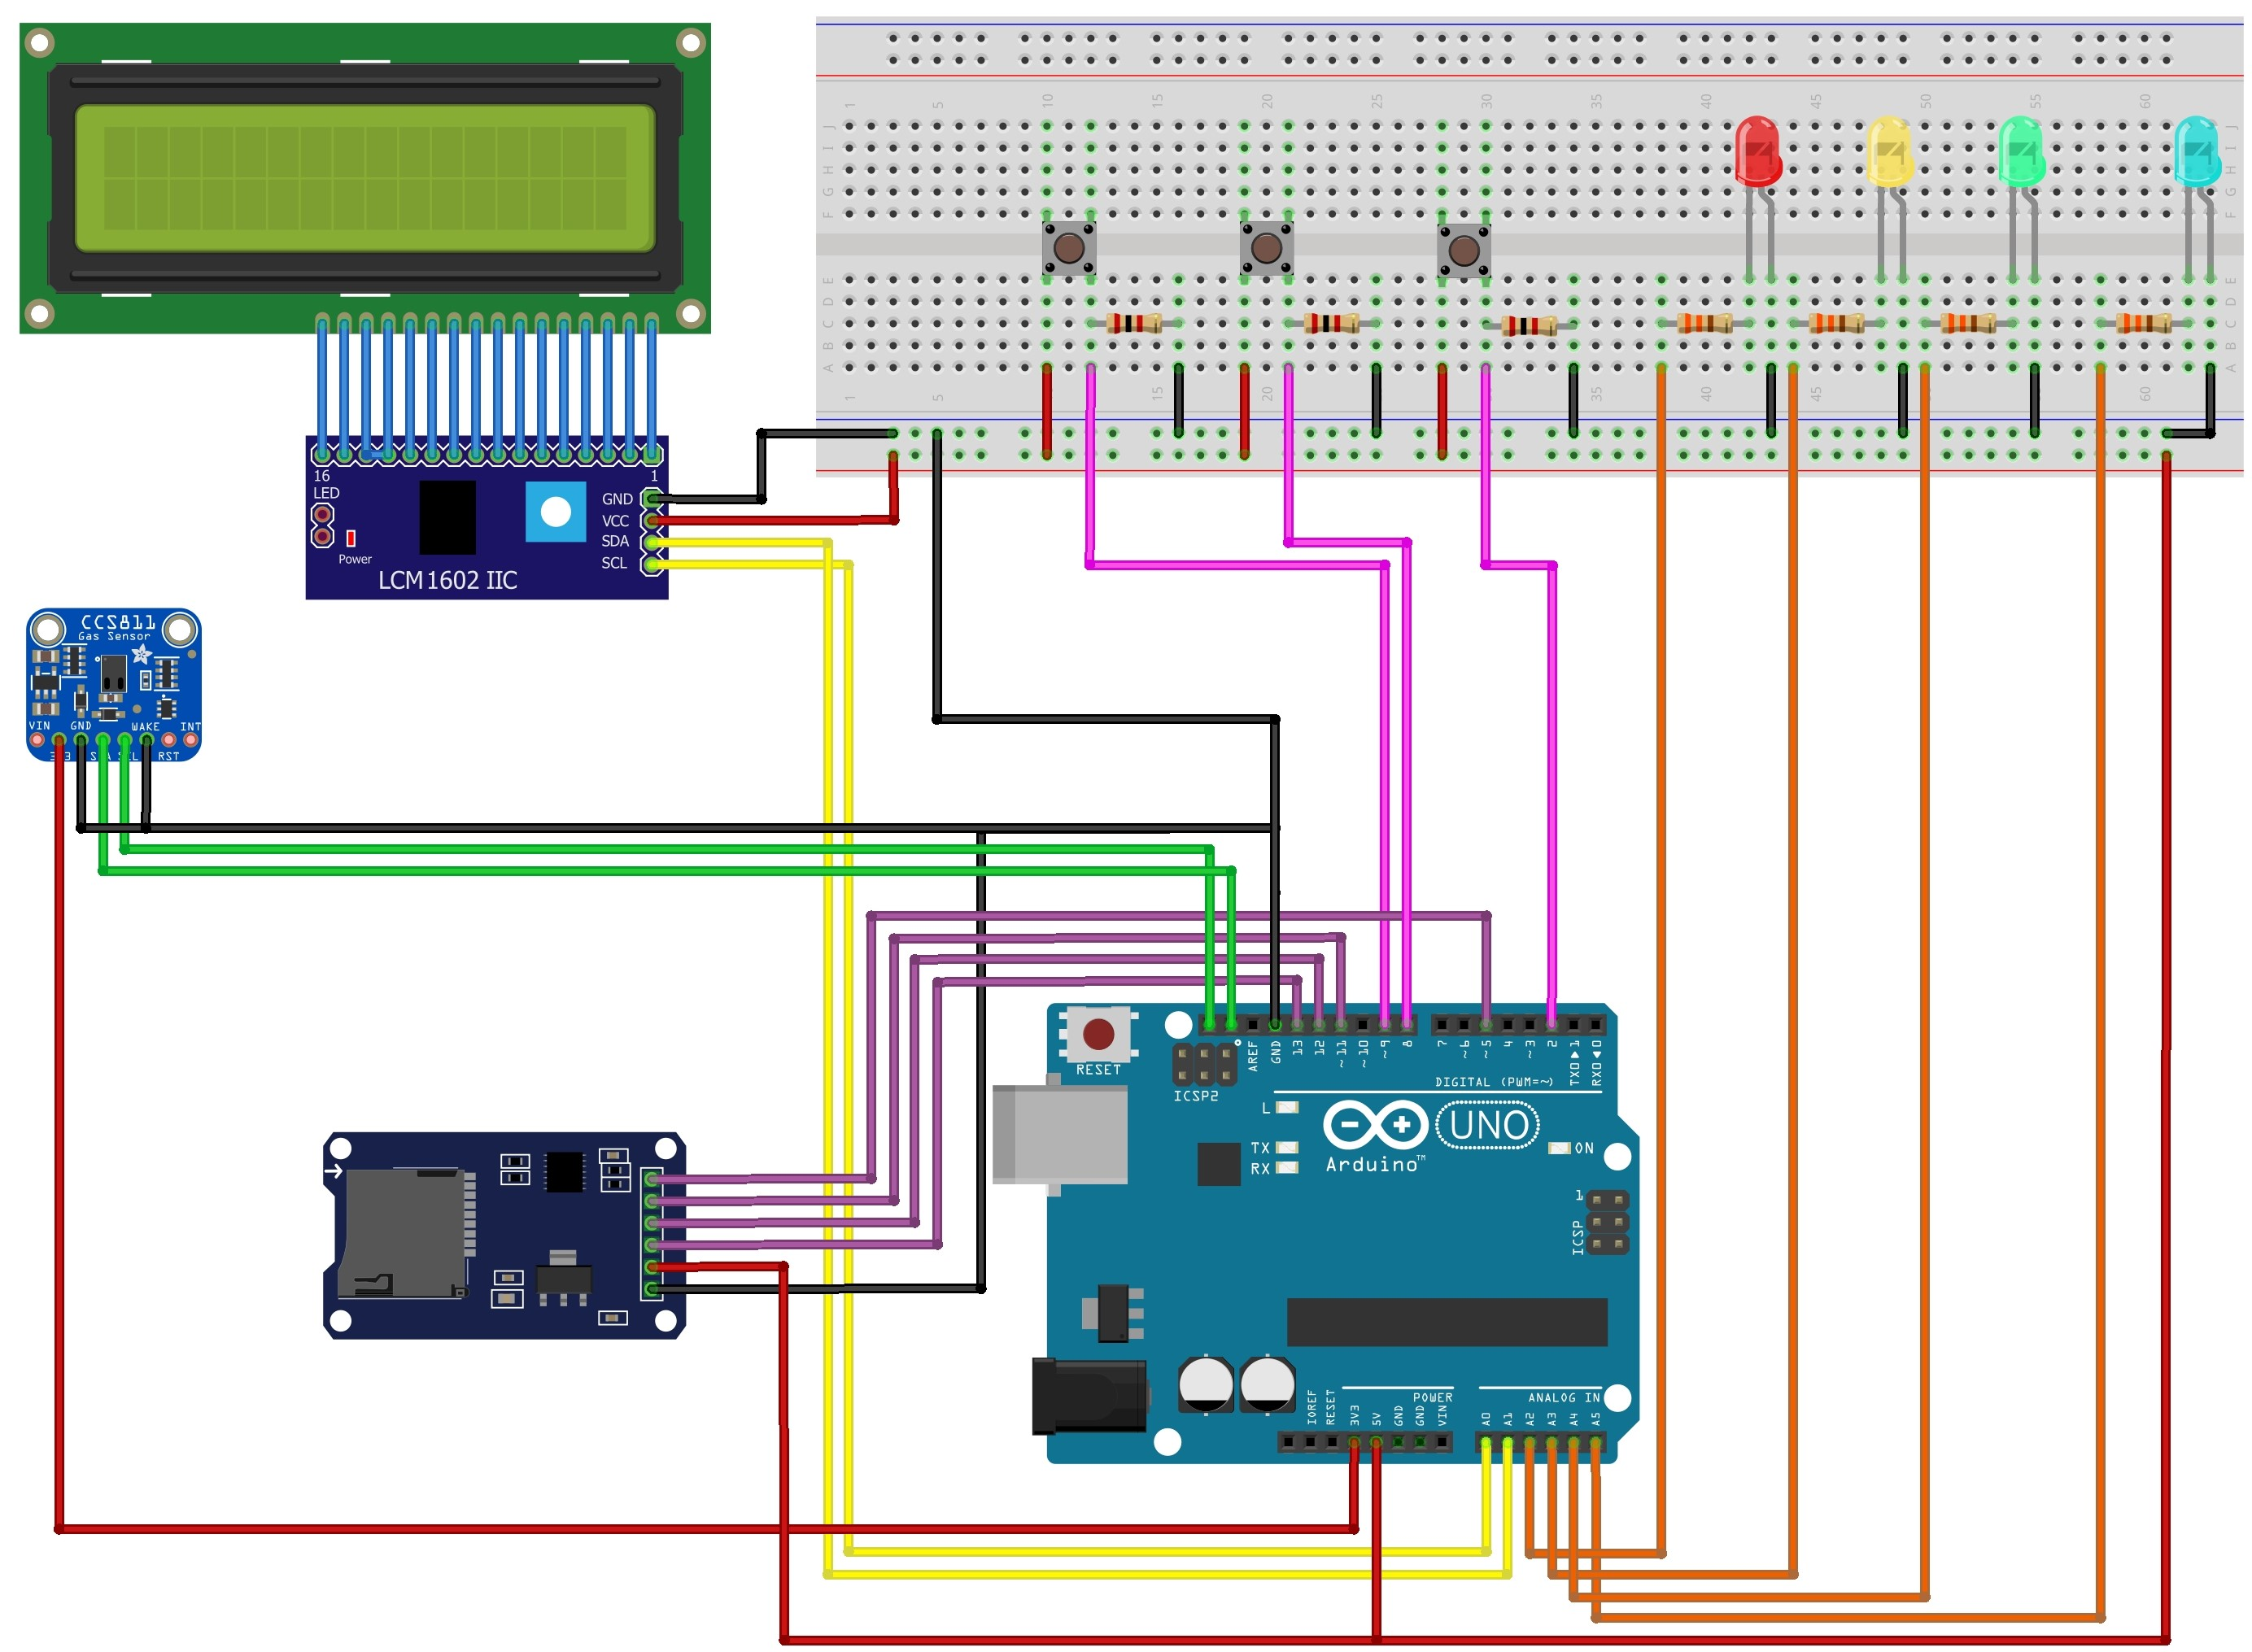
\includegraphics[width=0.9\linewidth]{Images/Layout_Steckplatine}
%	\caption{Entwurf der Toplevel-Architektur mithilfe von Enterprise Architect}
%	\label{fig:ToplevelArchitektur}
%\end{figure}

Damit der genaue Ablauf unseres Programms genau definiert ist, wurde, wie in \ref{fig:Statemachine} zu sehen ist, mithilfe von Enterprise Architect ein Zustandsdiagramm erstellt. \\

\begin{figure}[!hbt]
	\centering
	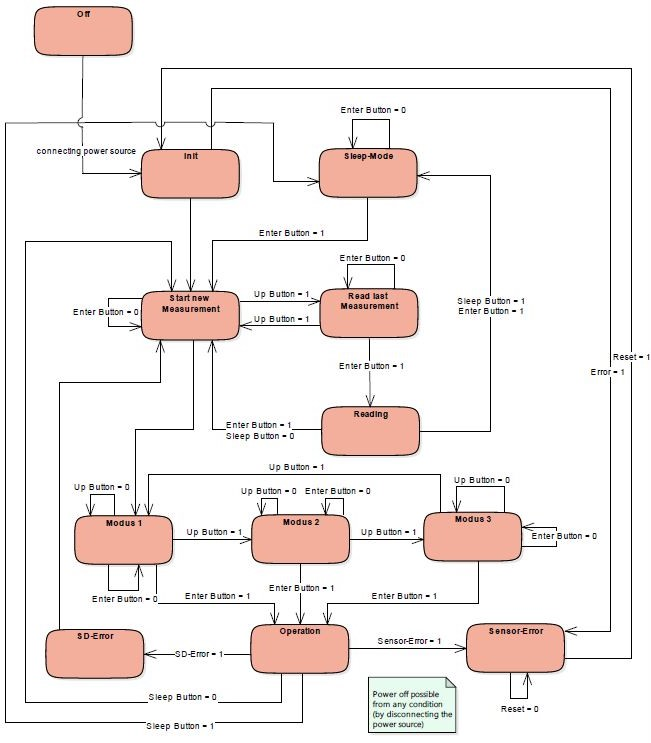
\includegraphics[width=0.9\linewidth]{Images/Statemachine}
	\caption{Entwurf des Zustandsdiagramms mithilfe von Enterprise Architect}
	\label{fig:Statemachine}
\end{figure}

Das Komponentendiagramm, welches in \ref{fig:KomponentenDiagramm} zu sehen ist, soll dazu dienen, alle Aktoren und deren Verbindungen darzustellen. \\

\begin{figure}[!hbt]
	\centering
	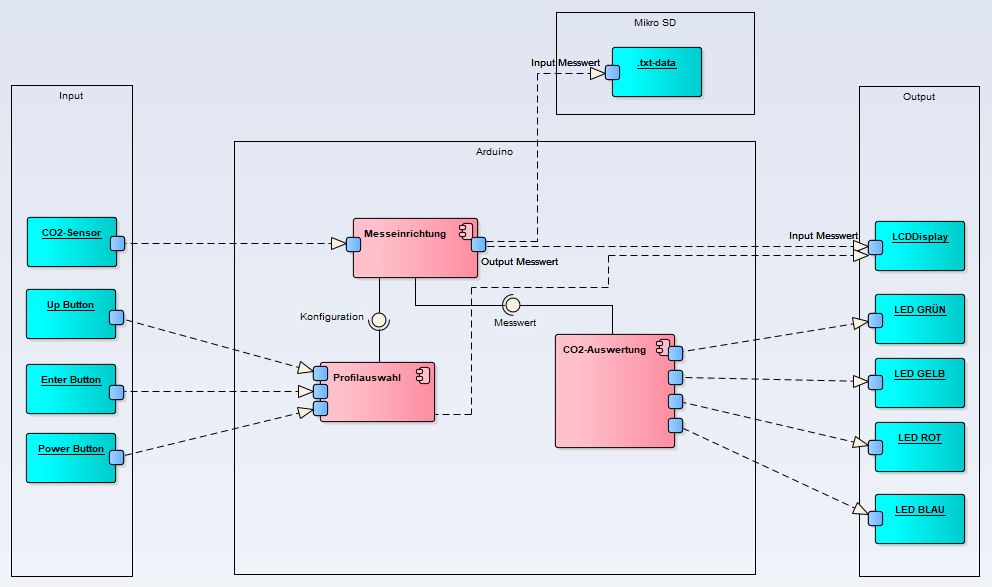
\includegraphics[width=0.9\linewidth]{Images/Komponentendiagramm}
	\caption{Entwurf des Komponentendiagramms mithilfe von Enterprise Architect}
	\label{fig:KomponentenDiagramm}
\end{figure}